\chapter{Problématiques émergentes \newline et orientations de recherche}

Dans ce mémoire, nous avons décrit divers modèles et principes de conception
d'un système sensible au contexte et présenté une multitude d'intergiciels et
d'approches distribuées pour simplifier la configuration d'applications
sensibles au contexte. De cet état de l'art se dégagent plusieurs problématiques
dans le développement d'un système de configuration basé sur le contexte
auxquelles nous tenterons d'apporter une solution.

\section{Intergiciel et détails d'implémentation}

Le besoin d'un nouvel intergiciel se fait ressentir du coté de l'implémentation.
Les technologies intergicielles actuelles ne sont pas adaptées pour le prise en
considération des restrictions imposées pas la mobilité et les systèmes
environnementaux intelligents : connexions volatiles, traitements et restrictions
mémoire sur les périphériques mobiles, canaux de communication étroits, écrans
réduits, mécanismes d'entrées restreintes, et la liste continue. Il existe
néanmoins une gamme d'implémentations de systèmes sensible au contexte dans la
littérature avec quelques prototypes fonctionnels :

\begin{itemize}
    \item \textbf{Hydrogen} \cite{hofer_context-awareness_2003}: 
        une architecture en trois couches.
    \item \textbf{Gaia} \cite{chetan_mobile_2005}: 
        une autre infrastructure intergicielle, étends les caractéristiques
        génériques des systèmes d'exploitation pour y incorporer la
        sensibilité au contexte.
    \item \textbf{CybreMinder} \cite{abowd_context-aware_2002}: 
        un système sensible au contexte permettant de générer des messages
        de rappel.
    \item \textbf{Context Toolkit} \cite{dey_conceptual_2001}: 
	    une architecture basée sur les widgets.
\end{itemize}

\section{Représentation des informations de contexte}

L'une des principales innovations à apporter dans les infrastructures
d'applications sensibles au contexte réside dans l'introduction d'une interface
présentant un niveau d'abstraction élevé. Cela permettrait de représenter la
connectivité des composants applicatifs avec les politiques de haut niveau qui
la régissent.Cette couche doit rester simple d'utilisation pour les
développeurs d'applications, et le modèle améliorer simultanément
l'automatisation et la sécurité.

\subsection{Ontologie de contexte}

La représentation des informations de contexte est grande préoccupation. Nous
avons présenté dans ce mémoire une approche basée sur les ontologie très
générique. Elle est basée sur quatre concepts fondamentaux : utilisateur,
environnement, plateforme et ressources. Actuellement, les ontologies sont
surtout utilisées pour permettre la communication entre les différents
périphériques dans le même réseau. Comme proposé par le ContextUML
\cite{sheng_contextuml:_2005}, le Langage de Modélisation Unifié (UML) peut
également être utilisé pour modéliser le contexte. Ces modèles pourraient être
utilisés pour séparer la définition et l'information liée au contexte de
l'implémentation spécifique. Il existe d'autres caractéristiques qui font que
l'information de contexte est difficile à modéliser : comme abordé précédemment,
il est parfois nécessaire de différencier une information statique d'une
information dynamique.

\subsubsection{Ontologie de services}

\begin{itemize}
  \item ServiceProfile (partie ''Quoi'')
  \item ServiceModel (partie ''Comment abstrait'')
  \item ServiceGrounding (partie ''Comment concret'')
\end{itemize}

Tout comme pour la standardisation de la gestion intelligente de la
configuration, la classe ServiceModel est très importante. Les services sont
modélisés comme des processus et la classe Process est utilisée pour indiquer
les opérations à des niveaux granularité différents. La classe Process comprend
principalement deux types de processus : atomiques et composites. Puisque
l'information de gestion de configuration est définie comme un ontologie OWL,
l'information peut être utilisée comme les paramètres des opérations de gestion
de la configuration, qui sont définis sous la forme de processus composites.
Chaque service de gestion de configuration correspond à un processus composite,
lui-même composé de plusieurs processus atomiques. Quand le gestionnaire invoque
un service de gestion de configuration prédéfini en OWL-S, le service sera alors
exécuté pour le dispositif réseau en place.

\section{Règles sémantiques et politiques de comportement}

Un autre domaine de recherche concernerait l'utilisation de règles pour exprimer
les comportements souhaités en termes d'éléments de haut niveau. Des langages
de définition de règles sont utilisés dans certains cas pour obtenir la
sensibilité au contexte. CRIME \cite{murphy_coordination_2007} par exemple, est
une implémentation prototypique du modèle Fact Space, qui est un langage de
coordination fournissant aux applications une vue de leur environnement. Les
règles CRIME décrivent le comportement des applications conformément à
l'information de contexte. CRIME traite également les déconnexions en invalidant
les faits et conclusions qui sont tirés des périphériques qui ne sont plus
disponibles dans l'environnement.

\subsection{Gestion basée sur des politiques (Policy-Based)}

La politique est identifiée comme une spécification de la configuration moyenne
du système sur des périodes persistantes. Un aspect important de cette
définition est qu'elle permet une certaine tolérance à l'erreur, nécessitée par
les évènements aléatoires se produisant susceptibles de corrompre la politique
en place dans la boucle de gestion du système. Il existe un élément probabiliste
ou stochastique pour le comportement du système et, par conséquent, la politique
ne peut être qu'une propriété moyenne en général.

\subsection{Modèle de définition des politiques d'administration}

Le modèle permettant la définition des politiques d'administration serait un
modèle orienté sur les ontologies et basé sur la théorie de la promesse.
Celle-ci s'appuie sur un contrôle évolutif des objets intelligents,
contrairement aux modèles impératifs plus traditionnels pensés comme des
systèmes de gestion descendants. Dans ces derniers, le gestionnaire central
doit être informé des commandes de configuration des objets sous-jacents et de
l'état actuel de ces objets.

Au sein du contexte, le modèle fournit une série d'objets qui définissent
l'application. Les objets englobent les terminaux, les groupes de terminaux et
les politiques qui définissent leurs relations.

L'infrastructure conçoit un modèle d'objet pour le déploiement d'applications,
ces dernières constituant le point central. Historiquement, les applications
étaient limitées par les capacités du réseau et par des configurations visant à
prévenir leur utilisation abusive. Des concepts tels que l'adressage, le VLAN et
la sécurité sont depuis toujours intrinsèquement liés, ce qui limite
l'évolutivité et la mobilité des applications. Alors que les applications sont
redessinées pour la mobilité et l'évolutivité web, cette approche traditionnelle
empêche leur déploiement rapide et homogène.

\subsection{Théorie de la promesse}

La théorie de la promesse est une théorie nouvelle sur ce qu'il peut arriver
dans un réseau de composants entièrement autonomes.

Plutôt que d'adopter la croyance conventionnelle que ''seulement ce qui est
programmé peut arriver'', elle pren le point de vue opposé : ''seulement ce
qui est promis peut être prédit''. Elle aborde donc la gestion du point de vue
de l'incertitude avec réalisme plutôt que celui de la foi en la conformité. Dans
la théorie de la promesse, on suppose un point de vue orienté service des
interactions entre les différents dispositifs informatiques. Chaque nœud propose
de jouer un rôle dans un réseau de collaboration en promettant de restreindre
son comportement de différentes manières. Une utilisation typique de la théorie
de la promesse est d'examiner le comportement en régime permanent d'un certain
nombre d'agents (composants) autonomes. La théorie de la promesse ne détermine
pas nécessairement pleinement le comportement de ses composants, elle représente
seulement les contraintes au sein d'un ensemble de comportements définis. Elle
n'est pas limitée aux promesses linéaires.

La théorie de la promesse adhère à un point de vue orienté service des
politiques des gestion et utilise un langage graphique pour composer et analyser
les propriétés systèmes.

Une caractéristique essentielle des promesses est qu'elles séparent clairement
ce qui contraint et à qui la contrainte s'applique. C'est un autre domaine qui
soulève bien souvent des confusions dans la théorie des politiques. Néanmoins,
le modèle ontologique permet un fois de plus de bien distinguer ces deux
aspects grâce à son haut degré de formalisme.

\subsubsection{CfEngine3: une implémentation de référence de la théorie de la
promesse}

CfEngine3 implémente deux approches :

\begin{itemize}
    \item \textbf{Centralisée}: 
        le système va pousser avec force les règles et règlements établis de
        manière centralisée avec ou sans la volonté de l'utilisateur final hôte.
    \item \textbf{Basé sur des politiques} :
        cette approche fonctionne de la même manière que le protocole SNMP
        (Simple Network Management Protocol), à l'exception qu'elle donne une
        autonomie totale aux agent, de manière à ce qu'ils aient plein droit de
        tirer et implémenter un ensemble centralisé de politiques de
        configuration.
\end{itemize}

En théorie, chacun des agents autonomes va faire formuler une promesse sur le
comportement qu'on attend de lui, basé sur un choix qui lui est propre. C'est ce
que rend la théorie de la promesse optimale pour un framework de gestion basé
sur des politiques.

La théorie de la promesse décrit des services régies par des politiques, dans un
framework d'agents complètement autonomes, qui s'aident les uns les autres
seulement par une coopération volontaire. Dans CfEngine3, chaque élément de
configuration va faire une promesse concernant ses caractéristiques propres et
sa relation avec d'autres éléments de configuration.

Nous souhaitons être en mesure de promettre que le système est cohérent, de le
vérifier et d'effectuer des changements seulement si nos promesses ne sont pas
tenues. Cela nécessite, en plus de l'implémentation initiale de ces promesses,
la vérification continue de l'état de chacun des éléments de configuration
vis-à-vis de leur promesses respectives pour assurer un système cohérent et en
conformité avec les politiques en vigueur.

% TODO : expliquer ITIL
%Pour comprendre ITIL (Information Technology Infrastructure Library), il
%faut l'imaginer comme un service fourni par CfEngine.

\subsubsection{Définition de la promesse}

Une promesse est différente d'un engagement : un engagement est le moment où un
agent rompt avec une ligne de conduite pour une autre discontinue avec des vues
sur un objectif, la plupart du temps à travers une action spécifique ou un
investissement sur des résultats futurs. Dans certains cas, l'acte
d'engagement peut résulter en une promesse persistante, mais promettre
n'implique pas une action provoquant un changement discontinu.

\begin{figure}[H]
    \centering
    \begin{tabular}{l}
        ``Une promesse est la spécification d'un état ou comportement \\
        ultérieur d'un agent autonome à un autre. Elle est ainsi, \\
        une unité de politique.`` \cite{burgess_modeling_2006} \\
        \em \footnotesize Mark Burgess, Alva Couch, Modeling Next Generation
        Configuration Management Tools, \\
        \em \footnotesize Pp. 131-147 of the Proceedings of LISA '06,
        Décembre 2006
    \end{tabular}
    \caption{La promesse par Burgess et al. (2006)}
    \label{fig:quote}
\end{figure}

Les promesses sont faites à un agent par un agent et sont modélisées par une
relation unidirectionnelle labellisée par un \emph{corps} de promesse qui
définit la substance de la promesse. Une promesse avec le \emph{corps}
\textbf{+b} est une déclaration pour ''donner'' un comportement d'un agent à un
autre, tandis qu'une promesse avec le \emph{corps} \textbf{-b} est la
spécification de quel comportement sera reçu, accepté ou utilisé d'un agent à
l'autre.

\subsubsection{Caractéristiques de la promesse}

Un promesse est l'annonce d'un fait ou d'un comportement d'un prometteur à un
promis, sous le regard d'un certain nombre de témoins (définissant le champ
d'application de la promesse), dont le résultat n'a pas encore été évalué.  On
distingue deux types de promesses :

\begin{itemize}
    \item Une promesse d'accepter de se comporter comme une autre. C'est
        essentiel pour la définition de groupes, de rôles ou de structures
        sociales avec un consensus de comportement (cf.
        section~\ref{sec:consensus})
    \item Une promesse d'utiliser la promesse d'un autre. C'est crucial pour les
        interactions client/serveur, les dépendances et les contrôles d'accès.
\end{itemize}

Un promesse présentes les caractéristiques suivantes :

\begin{enumerate}
    \item Il doit y avoir des agents pour qu'une promesse existe.
    \item Il doit y avoir un prometteur (ou agent source).
    \item Il doit y avoir un promis (ou agent destinataire), qui peut très bien
        aussi être la source.
    \item Il doit y avoir un \emph{corps} qui décrit la nature de la promesse.
\end{enumerate}

\subsubsection{Représentation et types de promesse: $\pi$-calculus}

\begin{table}[H]
    \begin{tabularx}{\textwidth}{
            >{\centering\arraybackslash}X|
            >{\centering\arraybackslash}X|
            >{\centering\arraybackslash}X|
        }

        \cline{2-3}
        & 
        \textbf{Notation} &
        \textbf{Interprétation} \\ 

        \cline{2-3}
        &
        $a \xrightarrow{+b} a'$ &
        Promesse avec le \emph{corps} $b$ \\

        &
        $a' \xrightarrow{-b} a$ &
        Promesse d'accepter $b$ \\

        &
        $v_a(a \xrightarrow{b} a')$ &
        La valeur de la promesse à $a$ \\

        \cline{1-1}
        \multicolumn{1}{ |X| }{\textbf{Type de promesse}} &
        $v_{a'}(a \xrightarrow{b} a')$ &
        La valeur de la promesse à $a'$ \\

        \cline{1-3}
        \multicolumn{1}{ |c| }{Basique} &
        $n_1 \xrightarrow{\pi} n_2$ &
        Fournit un service / un flux \\

        \multicolumn{1}{ |c| }{Coopérative} &
        $n_1 \xrightarrow{C(\pi)} n_2$ &
        Imite / Suit \\

        \multicolumn{1}{ |c| }{Utilisatrice} &
        $n_1 \xrightarrow{U(\pi)} n_2$ &
        Utilise / Accepte de la part de\\

        \multicolumn{1}{ |c| }{Conditionnelle} &
        $n_1 \xrightarrow{\pi_1/\pi_2} n_2$ &
        ``File`` de promesses: $\pi_1$ if $\pi_2$\\
        \cline{1-3}
    \end{tabularx}
    \caption{Représentation et types de promesses}
    \label{PromiseTypes}
\end{table}
   
Les promesses de services basiques forment un certain nombre de types, comme par
exemple `fournir un web service en moins de 5 millisecondes` ou `donner
n'importe quel information sur l'agent X`. D'autres exemples :

\begin{itemize}
    \item $X \xrightarrow{q \leq q_0} Y $: l'agent $X$ promet de ne jamais éxeder la
        limite $q \leq q_0$.
    \item $X \xrightarrow{q = q_0} Y $: l'agent $X$ promet de satisfaire
        $q = q_0$.
    \item $X \xrightarrow{\ell \subseteq  L} Y $: $X$ promet de garder $\ell$
        comme sous-langage du langage L
    \item $X \xrightarrow{S} Y $: $X$ offre le service $S$ à $Y$.
    \item $X \xrightarrow{R} Y $: $X$ promet de relayer $R$ à $Y$.
    \item $X \xrightarrow{\neg R} Y $: $X$ promet de ne jamais relayer $R$ à $Y$.
    \item $X \xrightarrow{S,t} Y $: $X$ promet de répondre avec le service $S$
        en l'espace de $t$ secondes.
\end{itemize}

Une promesse est dite ``rompue`` si un agent fait deux promesses différentes du
même type en même temps (différent d'une promesse qui aurait expiré ou changé).

\subsubsection{Processus de raisonnement lié à la promesse}

Le procédé de raisonnement qui accompagne l'émanation d'un promesse, se divisent
en plusieurs sous-étapes, accrochez-vous:

\begin{itemize}
  \item \textbf{Préparation de la promesse} :
	Processus de raisonnement effectué par A conduisant à la conception, la
	synchronisation et la délivrance de la promesse P par A.
  \item \textbf{Analyse de crédibilité} :
	Processus de raisonnement où les agents C dans le champ d'application de
	la promesse P déterminent la crédibilité qu'ils assignent à A promettant
	P compte tenu des faits connus de A (mais à l'exception des informations
	historiques précises sur le comportement individuel d'un membre de sa
	classe d'agent)
  \item \textbf{Détermination préliminaire de la confiance} :
	Processus de raisonnement effectué par C (C dans le domaine
	d'application de la promesse P) servant à :
  	\begin{enumerate}
	  \item Déterminer la confiance que C accorde à A avant même de
		  connaitre la promesse P (confiance préalable)
	  \item Spécifier quelles sont les attentes générées par la prise en
		  considération de la promesse P.
  	\end{enumerate}
  \item \textbf{Délibération de contre-promesse} :
	Processus de raisonnement effectué par B concernant les contre-promesses
	pouvant potentiellement être émises par B en retour de considération de
	P (B dans le champ d'application de P)
  \item \textbf{Prédiction de l'impact de la promesse} :
	(cela peut être réalisé à condition que B ait émis une ou plusieurs
	contre-promesses plausibles)
  	\begin{enumerate}
	  \item Processus de raisonnement effectué par B (dans le champ
		  d'application de P) et C (n'importe quel agent dans le champ
		  d'application de P) servant à déterminer les (le changement
		  des) attentes que P créé dans B (et que A a l'intention de
		  générer).  
	  \item Processus de raisonnement visant à la modification des ententes
		  (détenues par B ou C) étant donné la changement des attentes
		  de chacun d'entre eux amené par la prise en considération de
		  la promesse P.
  	\end{enumerate}
  \item \textbf{Évaluation de la promesse} :
	Processus de raisonnement effectué par C concernant :
  	\begin{enumerate}
	  \item La façon dont C va évaluer si la promesse de A a été tenue ou
		  non.
      \item L'évaluation de cette dernière au moyen de la méthode la plus
          adéquate
  	\end{enumerate}
  \item \textbf{Surveillance de rétraction de promesse} :
	A peut être amené à un stade ultérieur à émettre une autre promesse Q,
	pour laquelle la tenue n'est pas compatible avec la tenue de P. Dans ce
	cas, Q qualifie un retrait de P. Un agent C applique un processus de
	raisonnement qui surveille et évalue les promesses postérieures émises
	par A pour déterminer si celles-ci seront amenées à rompre la promesse P
	et induire sont retrait.
  \item \textbf{Mise à jour de la confiance} :
	Processus de raisonnement en place pour chacun des agents C dans le champ
	d'application de P visant à mettre à jour la confiance préalablement
	accordée à A, en adéquation avec la résultat de l'évaluation que C fait
	concernant le degré avec lequel la promesse P a été tenue par A.
  \item \textbf{Critère de réputation} :
	Processus de raisonnement effectué par chacun des agents C dans le champ
	d'application de P visant à échanger entre les différent agents les
	effets des mises à jour de confiance. Le flux de réputation permet a un
	agent C n'ayant aucuns aprioris sur un agent A d'acquérir une confiance
	initiale en prenant en considération les preuves recueillies par les
    autres agents (parce que même les agents ont des casiers judiciaires).
\end{itemize}

\subsection{Gestion de configuration basée sur la théorie de la promesse}

\subsubsection{Données paramètres}

Un système de gestion de configuration basé sur la théorie de la promesse
accepte comme paramètres d'entrée un ensemble de politiques de configuration de
haut niveau. Ces politiques de haut niveau seront divisées en spécifications de
configuration de bas niveau, que nous appellerons ``promesses`` dans la
modélisation par la théorie de la promesse. Notre ontologie permettra
formalisation de ces promesses.

En complément des politiques de configuration, les informations suivantes
pourront être transmises au système de gestion de configuration :

\begin{itemize}
    \item Le nombre et le type de machines nécessaires
    \item Le système d'exploitation de chacune des machines
    \item Les paquets ayant besoin d'être installés sur chaque machine
    \item Les services que chacun des hôtes doit fournir
    \item Les préoccupations liées au stockage comme le type de système de
        fichiers
    \item Les questions de sécurité, incluant notamment les aspect de gestion
        des utilisateurs
\end{itemize}

\subsubsection{Traitements}

Les politiques de configuration de haut niveau subirons deux traitements majeurs
:

\begin{enumerate}
    \item Spécification de la configuration de bas niveau. Ce traitement dépend
        de l'information liée à l'architecture telle que le détail du
        périphérique ou le type de topologie attendu par un système.
    \item Respecter les promesses formulées par chacun des éléments de
        configuration. Ce traitement consiste à ce que chaque élément de
        configuration se comporte conformément à leurs promesses. Dans la
        gestion des changements, CfEngine3 prendra des mesures correctives en
        plus de jouer le rôle d'informer les parties concernées en cas de non
        tenue d'une promesse.
\end{enumerate}

\subsubsection{Résultats attendus}

Le résultat de ces traitements est un système conforme aux règles politiques en
vigueur où chaque élément de configuration possèdent les clés et valeurs
attendues.  Autrement dit, un ensemble d'ordinateurs avec les valeurs de
configuration appropriées (les valeurs d'attribut promises).  Les éléments de
configuration principaux sont les fichiers, les paquets, les disques, les
processus, le services et les interfaces. 

En plus de leurs propres valeurs d'attributs et manière d'agir, un ensemble de
promesses sur le bon type de relations entre ces éléments de configuration est
nécéssaire pour valider le résultat de ces traitements.

\section{Consistance de l'information et tolérance à l'échec}

\subsection{Algorithme de consensus}
\label{sec:consensus}

Le consensus est un problème fondamental dans les systèmes distribués tolérants
aux pannes. Un consensus implique de multiples serveurs acceptant des valeurs.
Une fois qu'ils atteignent une décision sur une valeur, cette décision est
définitive. Les algorithmes de consensus typiques sont amenés à faire des
progrès lorsque la majorité de leurs serveurs sont disponibles, par exemple, un
cluster de 5 serveurs peut continuer à fonctionner même si deux serveurs ne sont
plus disponibles. Si plusieurs serveurs échouent, ils cessent de faire des
progrès (mais ils ne retournerons jamais de valeurs erronées).

\subsubsection{Pourquoi Raft ?}

Raft est un algorithme de consensus qui est conçu pour être facile à comprendre.
Il est équivalent à Paxos dans la tolérance aux pannes et en termes de
performance. La différence est qu'il est décomposé en sous-problèmes
relativement disjoints, et traite de manière rigoureuse toutes les pièces
majeures nécessaires pour obtenir un système cohérent.

Il existe des écarts significatifs entre la description de l'algorithme de Paxos
et les besoins d'un système dans le monde réel. Le système au final serait basé
sur un protocole dénué de preuves.

\begin{tabular}{p{.48\textwidth}p{.48\textwidth}}
    \noindent
    \textbf{\textit{Inconvénients de Paxos}}

    \begin{itemize}
        \item Extrêmement difficile à comprendre. L'opacité de Paxos dérive de
            son choix d'avoir un sous-ensemble de décrets uniques comme son
            fondement.
        \item Ne fourni pas une bonne base pour la construction d'applications
            pratiques. Par exemple, il y peu d'avantages à choisir de manière
            indépendante une collection d'entrées dans le registre, pour les
            fusionner par la suite dans un journal séquentiel ; cela ajoute
            juste de la complexité. Il est plus simple et plus efficace de
            concevoir un système autour d'un journal, où les nouvelles entrées
            sont ajoutées séquentiellement dans un ordre contraint.
        \item Utilise une approche symétrique pair-à-pair à sa base. Cela a un
            sens dans un monde simplifié où seule une décision sera prise, mais
            peu de systèmes concrets utilisent cette approche.  Si une série de
            décisions doivent être prises, il est plus simple et plus rapide
            d'élire d'abord un leader, puis de le laisser coordonner les
            décisions.
    \end{itemize} 
    
    &

    \textbf{\textit{Avantages de Raft}}

    \begin{itemize}
        \item Raft utilise une forme plus solide de leadership que les autres
            algorithmes de consensus. Par exemple, les entrées du registre de
            seront communiquées que par le leader vers les autres serveurs. Cela
            simplifie largement la gestion de la réplication des journaux et
            rend Raft beaucoup plus facile à comprendre.
        \item Raft utilise des minuteries aléatoires pour élire les leaders.
            Cela ajoute un peu de mécanismes au système de pulsation déjà
            nécessaire dans n'importe quel algorithme de consensus, tandis que
            la résolution des confits se fait simplement et rapidement.
        \item Le mécanisme de Raft pour changer l'ensemble des serveurs de la
            grappe utilise une nouvelle approche de consensus conjointe où les
            majorités des deux différentes configurations se superposent pendant
            les transitions. Cela permet au groupe de continuer à fonctionner
            normalement pendant les changements de configuration.
    \end{itemize}

\end{tabular}

\subsubsection{Architecture de machines à états répliquées}

\begin{wrapfigure}{r}{.5\textwidth}
    \centerline{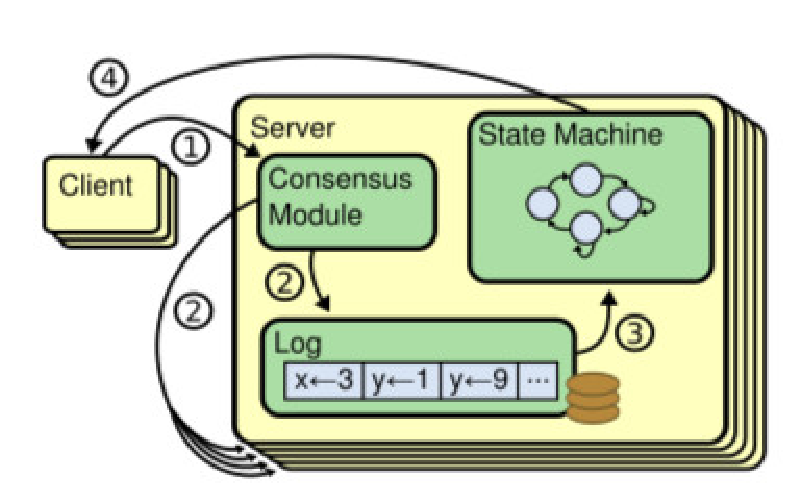
\includegraphics[width=.47\textwidth]{img/replicated_state_machine}}
    \caption{Procédé de réplication des machines à états}
    \label{replicated_state_machine}
\end{wrapfigure}

L'algorithme de consensus gère un registre répliqué contenant les commandes de
la machine à états de chacun des clients dans le réseau. Les machines à états
traitent des séquences identiques de commandes à partir de journaux partagés, de
sorte qu'ils produisent les mêmes résultats.

Les systèmes à grande échelle n'ayant qu'un seul cluster leader utilisent une
machine à état distincte pour gérer les élections et pour stocker les
informations de configuration qui doivent survivre aux crashs du leader
(exemple: Chubby, ZooKeeper).

\begin{verse}
    \underline{
        Garder le registre répliqué consistant est le travail de l'algorithme de
        consensus.
    }
\end{verse}

Les algorithmes de consensus pour les systèmes concrets ont généralement les
caractéristiques suivantes :

\begin{itemize}
    \item Ils assurent la sécurité (ne retournent jamais de résultat erroné)
        sous toutes conditions non byzantines, y compris les retards dans le
        réseau, les pertes de partitions et de paquets, la duplication et
        la réorganisation.
    \item Ils sont entièrement fonctionnels (disponibles) dans la mesure où au
        moins la majorité des serveurs sont opérationnels et peuvent communiquer
        avec les uns les autres et avec les clients. Ainsi, un groupe type de
        cinq serveurs peut tolérer la défaillance de deux ses membres. Les
        serveurs sont supposés tomber en panne en s'arrêtant ; ils pourront plus
        tard retrouver un état stable et rejoindre le cluster.
    \item Il ne dépendent pas de la contrainte temporelle pour assurer la
        cohérence des journaux : des horloges défectueuses et des retards
        abusifs dans la délivrance des messages peuvent causer des problèmes de
        disponibilité. 
    \item Dans le cas le plus courant, une commande peut s'achever aussitôt que
        la majorité de la grappe a répondu à un seul tour d'appels à procédures
        distantes ; une minorité de serveurs lents de doivent pas impacter les
        performances globales du système.
\end{itemize}

\subsubsection{États des serveurs}

Un cluster Raft comprend une multitude des serveurs (cinq est un nombre courant
permettant au système de tolérer deux échecs). À n'importe quel moment donné,
chacun des serveur est dans l'un de ces états :

\begin{wrapfigure}{r}{.5\textwidth}
    \centerline{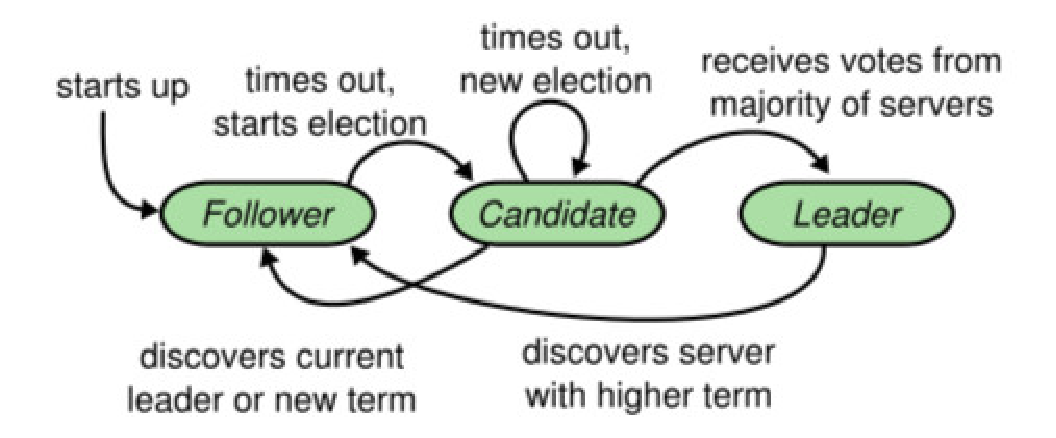
\includegraphics[width=.47\textwidth]{img/raft_server_states}}
    \caption{États et transitions dans un cluster Raft}
    \label{raft_server_states}
\end{wrapfigure}

\begin{itemize}
    \item \textbf{Leader} :
        En cycle normal, il existe un et un seul \emph{leader} et tous les autres
        serveurs sont \emph{followers}. Le \emph{leader} traite les requêtes de
        tous les clients (si un client contact un \emph{follower}, le
        \emph{follower} le redirige vers le \emph{leader}).
    \item \textbf{Follower} :
        Les \emph{followers} sont passifs : ils n'émettent jamais de messages par
        leur propre initiative, ils se contentent simplement de répondre aux
        requêtes émises par le \emph{leader} et les \emph{candidats}.
    \item \textbf{Candidat} :
        Statut intermédiaire utilisé lors de l'élection d'un nouveau
        \emph{leader}. La figure \ref{raft_server_states} montre les différents états
        et transitions possibles dans le consensus de Raft.
\end{itemize}

Les \emph{followers} ne font que répondre aux requêtes des autres serveurs. Si
un \emph{follower} ne reçoit plus de communications, il devient alors
\emph{candidat} et initie une élection. Le \emph{candidat} qui reçoit les votes
d'un majorité du cluster complet devient le nouveau \emph{leader}. D'une manière
générale, les \emph{leaders} opèrent jusqu'à ce qu'ils échouent.

\section{Conclusion}



% ex: set spelllang=fr spell: %
%%% Local Variables: ***
%%% mode: latex ***
%%% TeX-master: "thesis.tex" ***
%%% End: ***
